Para acceder a la herramienta \emph{MenuStrip} se selecciona la opción correspondiente en la \emph{ToolBox}.

\begin{figure}[H]
  \centering
  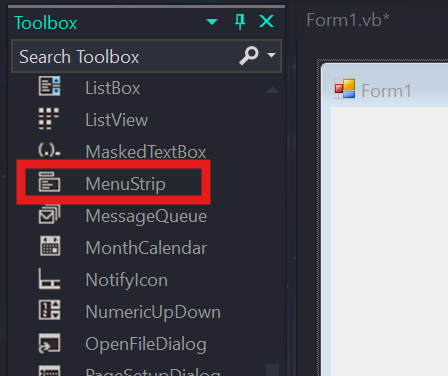
\includegraphics[scale = 1]{Imagenes/manual_1.png}
  \caption{Herramienta MenuStrip}{Fuente: Propia}
\end{figure}

En la ventana del \emph{Form} aparece en la parte superior el \emph{MenuStrip}.

\begin{figure}[H]
  \centering
  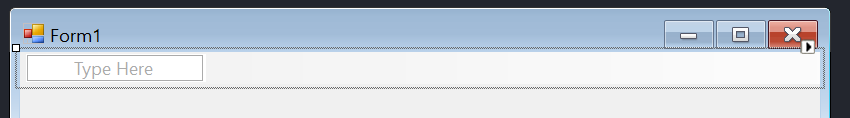
\includegraphics[scale = 0.7]{Imagenes/manual_2.png}
  \caption{MenuStrip en la ventana Form}{Fuente: Propia}
\end{figure}

Se puede inidcar el nombre del \emph{menú desplegable} y los \emph{submenús} que conforman la interfaz.

\begin{figure}[htb]
  \centering
  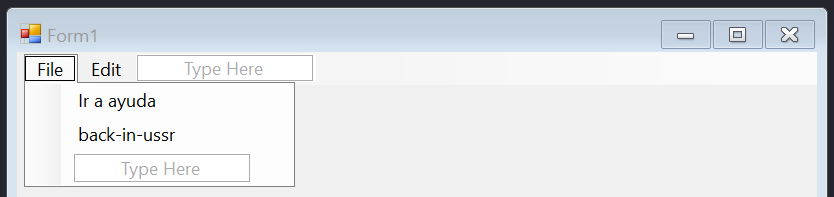
\includegraphics[scale = 0.6]{Imagenes/manual_3.png}
  \caption{Menú desplegable}{Fuente: Propia}
\end{figure}

Se puede programar la acción que ejecuta cada \emph{submenú} haciendo doble click izquierdo sobre el mismo.

\begin{figure}[htb]
  \centering
  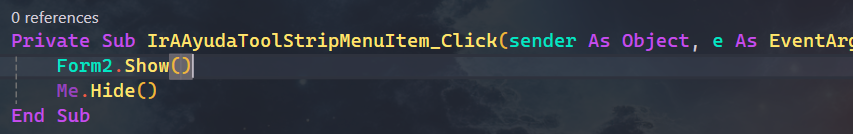
\includegraphics[scale = 0.6]{Imagenes/manual_4.png}
  \caption{Programación de submenú}{Fuente: Propia}
\end{figure}